\chapter{Referencial Teórico}
\label{cap:referencial-teorico}

  Neste capítulo esclarecemos os conceitos teóricos necessários para o
entendimento do trabalho e a metodologia proposta. Inicialmente, abordamos
aspectos da visualização de dados de tráfego e formas comuns de representação
dessa informação.  Neste contexto, destacamos os problemas para representar
uma grande quantidade de dados e alternativas para solucioná-los. Por fim,
apresentamos os dados da pesquisa do metrô que iremos utilizar.

\section{Visualização de Dados de Tráfego}
\label{sec:viz-trafego}

A análise de dados do tráfego tem um histórico antigo. \citet{Chen2015} fazem
um levantamento de várias pesquisas de análise e visualização de dados do
tráfego de pessoas, carros e embarcações. Os trabalhos levantados abrangem problemas
diferentes em quatro categorias principais, conforme o seu objetivo e a tarefa a que servem.

Uma categoria são as de aplicações que focam no monitoramento do tráfego,
muitas vezes feito em tempo real para a descoberta instantânea de eventos,
geralmente com a coleta de dados através de câmeras e sensores que alimentam
sistemas de alerta.  Uma outra categoria são as das aplicações de exploração e
predição, que permitem que usuários investiguem os dados para justificar
situações do tráfego, como a ocorrência de congestionamentos devido a um alto
número de veículos, ou ainda prever tais situações com técnicas de predição
(e.g.  predizer que haverá congestionamento devido a ocorrência de chuva).  Há
também a classe de soluções voltadas para o planejamento e recomendação de
rotas, que podem envolver tanto o monitoramento em tempo real quanto análise
histórica no processo de recomendação. Por fim, \citet{Chen2015} cita a
categoria de aplicações voltadas para a descoberta de padrões e tendências de
mobilidade, que utilizam técnicas de agrupamento dos dados.

No contexto das aplicações para a descoberta de padrões e tendências, um
conjunto de dados pré estabelecido é analisado para se chegar a alguma
conclusão sobre suas características. Tratando-se de dados de tráfego, suas
características espaciais e temporais muitas vezes requerem abordagens
diferentes na investigação dos padrões e na construção de uma visualização. 

\subsection {Visualização das Propriedades Temporais}
\label{sec:prop-temporais}

Dados do tráfego podem conter uma série de variáveis, das quais as mais
importantes são o tempo e espaço. Visualizações orientadas ao tempo enfatizam
tendências, periodicidades e anomalias nos dados ao longo de um eixo temporal \citep{Aigner2008}.

Expressar a variação do tráfego ao longo do tempo e sua evolução é um típico
processo de análise linear do tempo, que é considerado a partir de um ponto de
início até um ponto final \citep{Chen2015}. Por exemplo, em um gráfico de
linhas, o tempo é representado ao longo do eixo X e outra variável é
representada no eixo Y, como na Figura \ref{fig:linear-time}. Gráficos de
linhas são fáceis de interpretar, porém limitam-se na quantidade de variáveis
que podem ser visualizadas.

\begin{figure}[!htb]
  \centering
  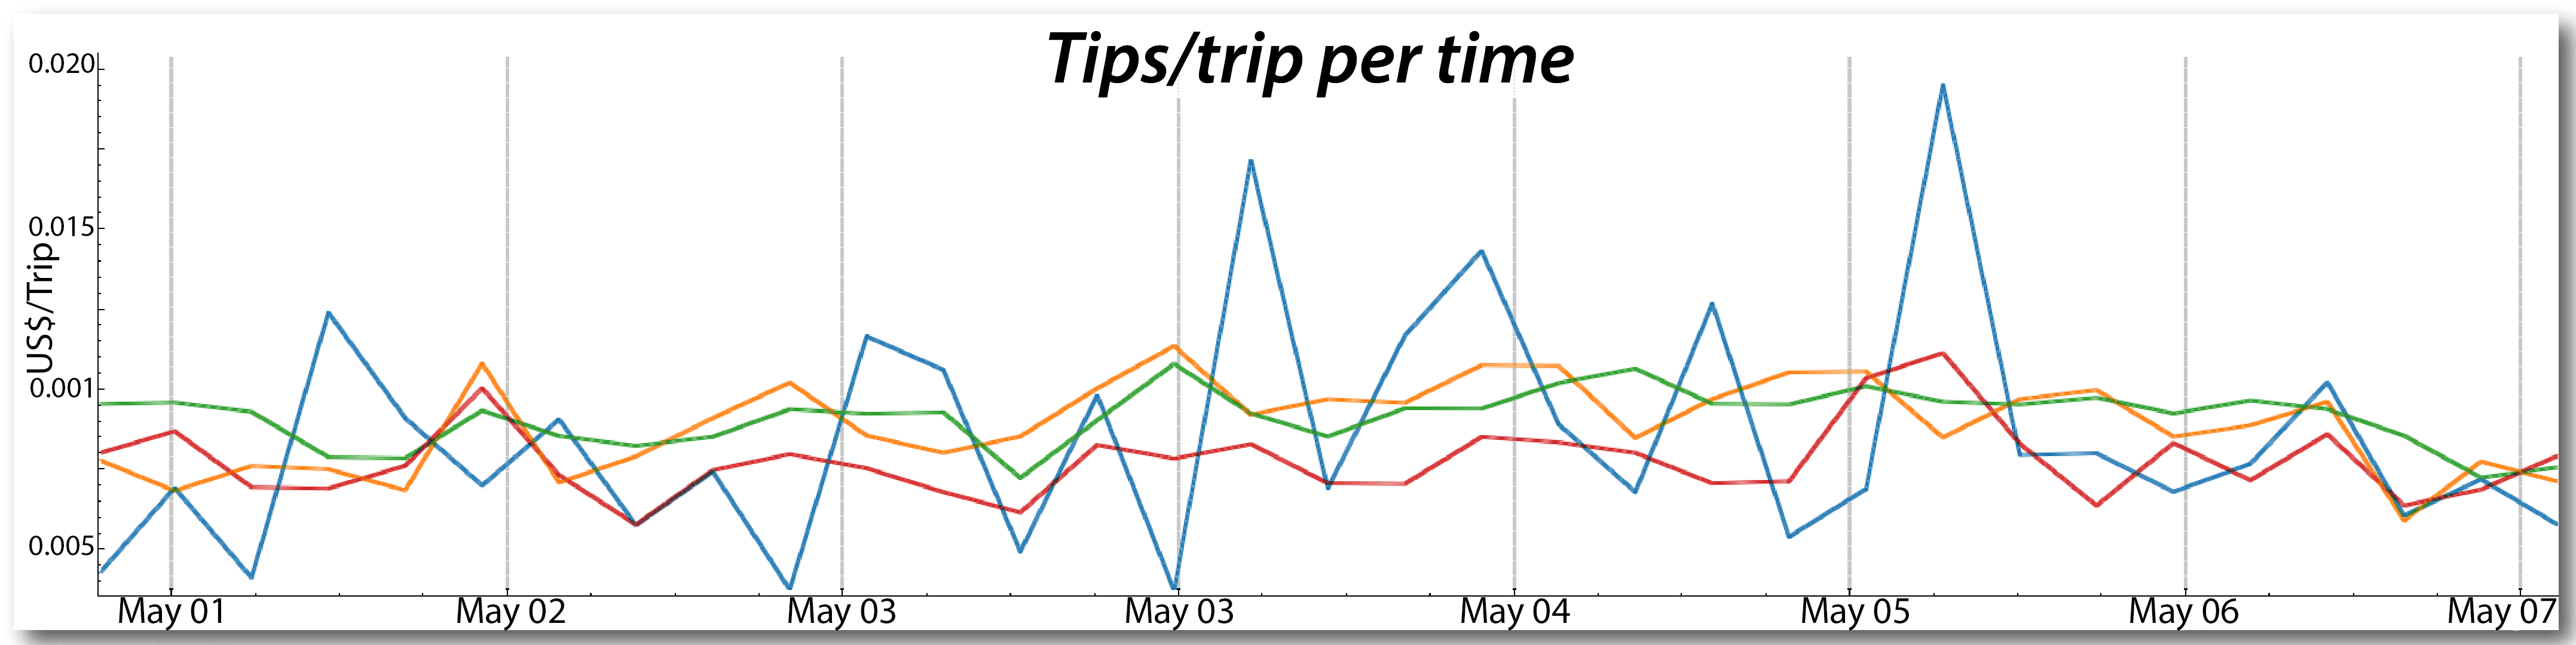
\includegraphics[width=\textwidth]{../figuras/linear-time.png}
  \caption[Gráfico de linha representando empo linear]{Gráfico de linha representando tempo linear. Ele mostra a média de gorjetas por viagem em diferentes regiões no período de 1 a 7 de Maio de 2011. Cada linha representa uma região. Fonte: \citep{Ferreira2013}
  \label{fig:linear-time}}
\end{figure}

  Por outro lado, temos também alguns processos recorrentes que são naturais em
nosso mundo, os quais seguem ciclos de estações, ou mesmo ciclos semanais e
diários. Um leiaute radial visto na Figura \ref{fig:periodic-time} é uma opção
para se visualizar essa periodicidade. O tempo é mostrado no eixo circular e
cada anel do círculo representa um dia da semana.  Os setores representam uma
hora, com 24 setores no total que mostram a quantidade de tráfego em um
determinado ponto da cidade, mapeada em cores. A vantagem de um leiaute radial
é que ele evidencia esses padrões recorrentes e a desvantagem é que ele possui
pouca eficiência espacial \citep{Chen2015}.

\begin{figure}[!htb]
  \centering
  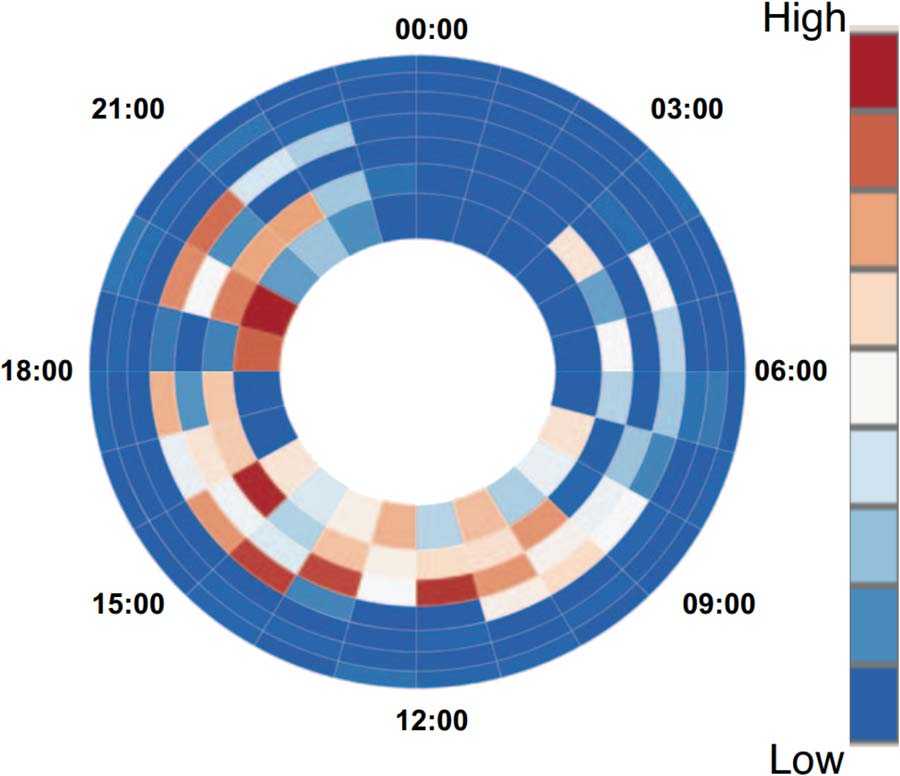
\includegraphics[width=0.6\textwidth]{../figuras/periodic-time.png}
  \caption[Leiaute radial representando tempo periódico]{Leiaute radial
representando tempo periódico. O tempo é mostrado no eixo circular e cada anel
do círculo representa um dia da semana, divididos em 24 setores que indicam as
24 horas do dia. As cores mostram a quantidade de tráfego conforme o mapa à
direita, onde vermelho maior é o tráfego. Fonte:
\citet{Pu2013} \label{fig:periodic-time}}
\end{figure}

  Os aspectos temporais dos dados não se limitam a apenas essas visualizações,
existe um grande arcabouço de projeções que se desenvolveram no campo da
visualização da informação onde o tempo é uma variável de destaque,
\citet{Cairo2016} mostra uma série dessas projeções em seu livro. Uma análise
linear ou periódica são dois paradigmas que levam a decisões diferentes durante
o processo de criação da visualização.

\subsection{Visualização das Propriedades Espaciais}
\label{sec:prop-espaciais}

  As propriedades espaciais de localização referem-se aos locais onde ações,
incidentes e eventos ocorrem. Diferentes níveis de agregação dessa informação
levam à categorização da visualização em três classes, segundo
\citet{Chen2015}: visualização baseada em pontos (nenhuma agregação),
visualização baseada em linhas (agregação de primeira ordem), e agregação
baseada em regiões (agregação de segunda ordem).

\begin{description}
  \item[Visualização baseada em pontos:] visualizações baseadas em pontos
consideram as informações do tráfego como pontos discretos e usam sua forma
pura como representação em um leiaute espacial, como por exemplo pontos em um mapa 2D. Essa técnica
mostra intuitivamente a posição de objetos em um certo momento no tempo. O
projeto \emph{Trains of Data}, ilustrado na Figura \ref{fig:trains-of-data},
utiliza esse tipo de visualização para representar a movimentação dos trens na
França. O tamanho dos pontos indica a quantidade de passageiros e a cor indica
se o trem está atrasado, sendo verde no horário e vermelho significa atraso.
Para uma visualização integral da trajetória eles ainda usam efeitos de
animação. Visualizações baseadas em pontos tipicamente representam cada ponto
de forma individual. Em casos onde há uma grande quantidade de pontos, o uso de
mapas de calor é indicado para a visualização da densidade. A vantagem desse
método é que ele permite observar os estados de cada objeto e sua distribuição
no espaço, como também explorar regiões da cidade que estejam mais ocupadas.
Por outro lado, ele é inapropriado para representação de informações contínuas,
como quantos veículos viajam de um determinado local para outro.

\begin{figure}[!htb]
  \centering
  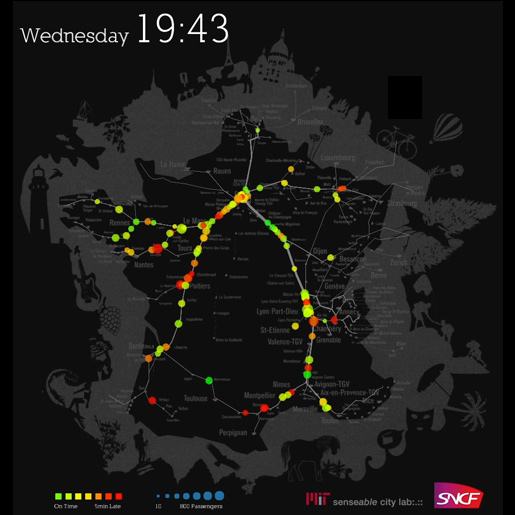
\includegraphics[width=.6\textwidth]{../figuras/trains-of-data.jpg}
  \caption[Visualização baseada no mapa das ferrovias da França]{Posição dos trens às 19:43 na França com uma visualização baseada no mapa
das ferrovias. Fonte: \citet{Senseable2018}.}
  \label{fig:trains-of-data}
\end{figure}

  \item[Visualização baseada em linhas:] visualizações baseadas em linhas são
desenhadas para mostrar a trajetória de objetos, mapas de vias e estradas em
uma região, ou fluxos do tráfego em uma rede de transporte. As trajetórias e
fluxos são representados por linhas ou curvas e são escaladas ou coloridas de
acordo com suas propriedades (i.e. densidade, direção, velocidade).
\citet{Klein2014} apresenta um sistema iterativo para análise do tráfego aéreo
na França. Cada trajetória é representada por uma linha que conecta os pontos
de partida e chegada de cada voo, como pode ser visto na Figura
\ref{fig:air-traffic}.

\begin{figure}[!htb]
  \centering
  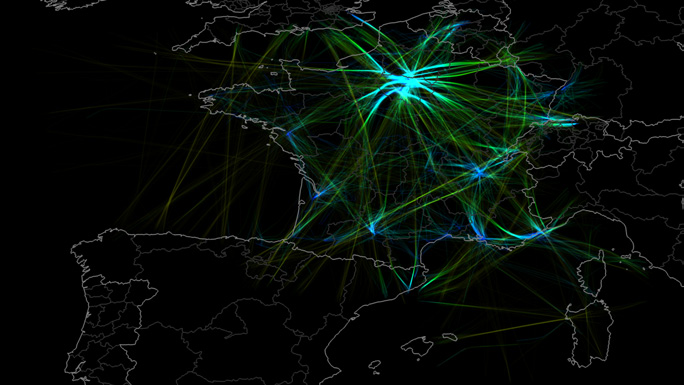
\includegraphics[width=1\textwidth]{../figuras/air-traffic.png}
  \caption[Visualização do tráfego aéreo na França]{Visualização do tráfego aéreo na França. Fonte: \citet{Klein2014}.}
  \label{fig:air-traffic}
\end{figure}

  A representação espacial das linhas pode ainda sofrer transformações
geométricas e topológicas que geram novas abstrações. Por exemplo,
\citet{Tarik2009} mostram uma proposta que transforma as trajetórias de um
leiaute espacial (Figura \ref{fig:viz-espacial}) para um leiaute abstrato
(Figura \ref{fig:viz-abstrata}) para visualizar a movimentação de pessoas
durante a fuga de uma explosão em um escritório.  A abordagem abstrata é usada
para mostrar mais efetivamente os padrões de movimentação de pessoas que se
movem ao mesmo tempo para as mesmas áreas. Na Figura \ref{fig:viz-abstrata} é
possível notar a movimentação de indivíduos antes da explosão (linhas azuis), o
que sugere possíveis suspeitos ou testemunhas do evento.  As informações
temporais são difíceis de representar no leiaute espacial, assim o leiaute
abstrato complementa a visualização dos dados mostrando os instantes de tempo
no eixo X e as informações espaciais no eixo Y.

\begin{figure}[ht!]
  \centering
  \begin{subfigure}[t]{0.45\textwidth}
    \centering
    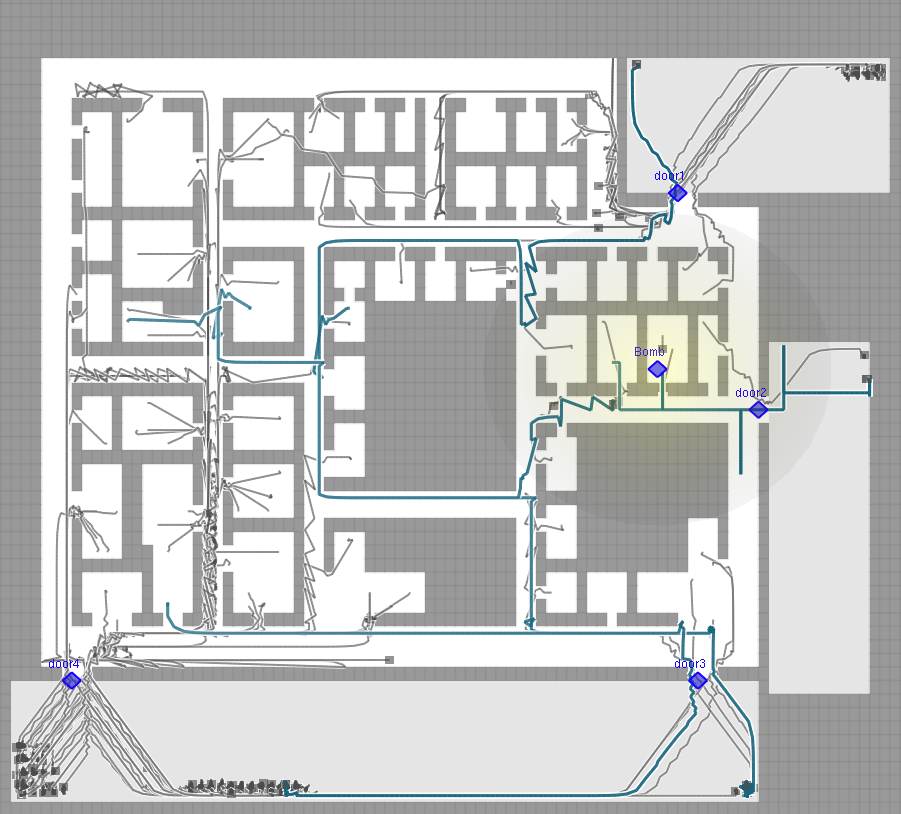
\includegraphics[width=65mm]{../figuras/proximidade-espacial.png}
    \caption{Visualização espacial das trajetórias ao longo do tempo. \label{fig:viz-espacial}}
  \end{subfigure}
  ~
  \begin{subfigure}[t]{0.45\textwidth}
    \centering
    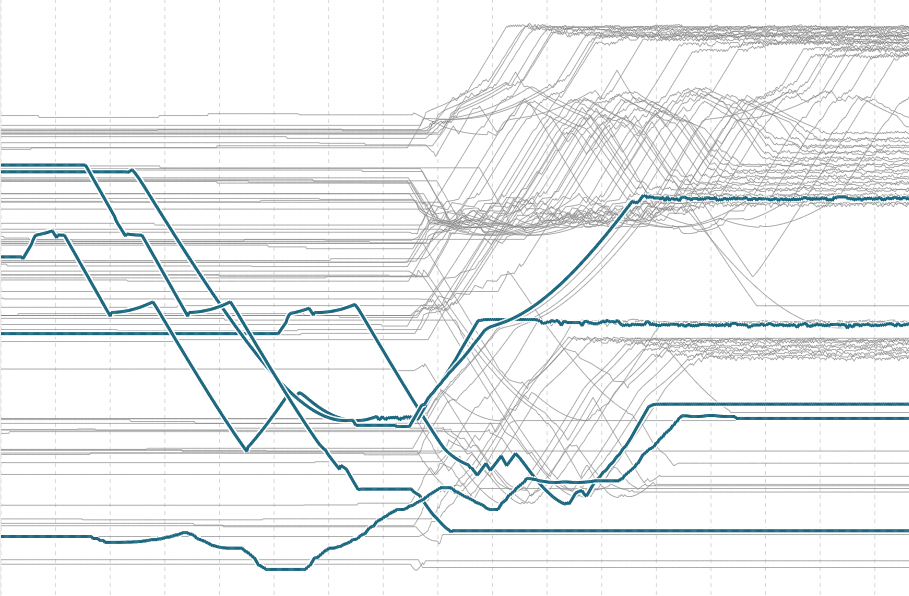
\includegraphics[width=75mm]{../figuras/proximidade-abstrata.png}
    \caption{Visualização abstrata da movimentação ao longo do tempo. \label{fig:viz-abstrata}}
  \end{subfigure}

  \caption[Visualização espacial vs abstrata da movimentação de pessoas]{Simulação de uma evacuação de um escritório depois de uma explosão.
(a) Visualização da movimentação da trajetória das pessoas no espaço. (b)
Visualização abstrata, baseada na proximidade.  Fonte: \citet{Tarik2009}.
\label{fig:tarik}}
\end{figure}

%  Algumas ideias buscam ainda sintetizar as informações espaciais e temporais
%em um cubo espaço-temporal, que utiliza o eixo Z para mostrar o tempo e os
%eixos X e Y para representar o espaço.

  No entanto, a medida que o número de objetos cresce, aumenta também os
problemas de oclusão, o que acaba afetando a estética da visualização e a
obtenção de informações sobre os dados \citep{Zhou2013}. Uma forma de reduzir
a complexidade de análise de um grande conjunto  trajetórias é utilizando
outras formas de abstração dos dados, como uma visualização baseada em regiões.

  \item[Visualização baseada em regiões:] Esse tipo de abstração agrupa fluxos
de deslocamento com origem e destino similares em um nível de macro regiões,
geralmente determinado por divisões administrativas.  \citet{Zeng2013}
apresentam um diagrama em círculos para mostrar padrões de movimentação de
pessoas entre as regiões da cidade. O círculo representa a junção ou conexão
entre as diferentes regiões e o fluxo entre elas. A densidade do fluxo é medido
pela espessura, bem como a direção é destacada dentro do círculo, como é
ilustrado na Figura \ref{fig:interchange-circo}. Apesar de facilitar a
visualização, esse tipo de agregação abre mão das informações individuais de
cada trajetória em favor de uma visão condensada dos fluxos.

\begin{figure}[!h]
  \centering
  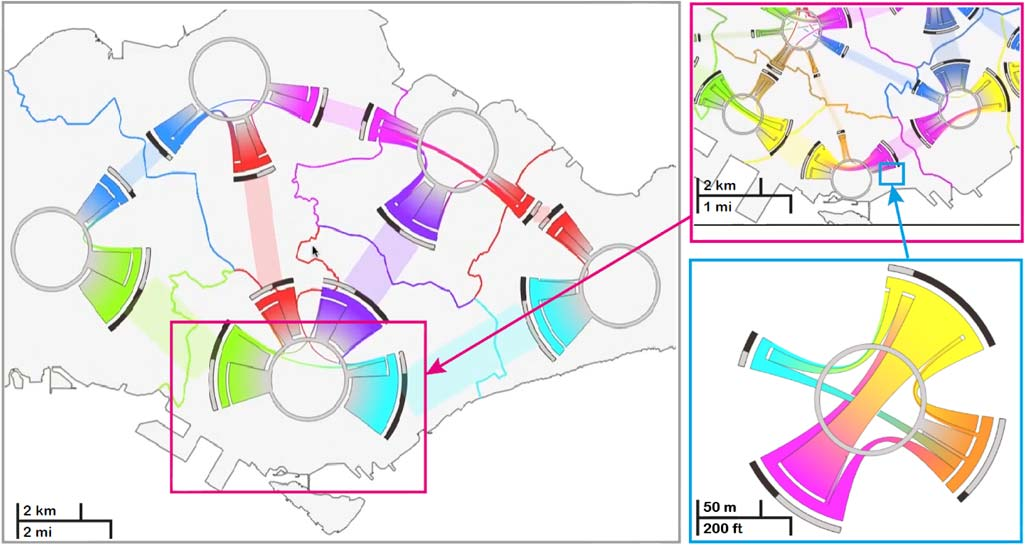
\includegraphics[width=0.97\textwidth]{../figuras/region-based.png}
  \caption[Exemplo de visualização baseada em regiões do sistema de metrô na França]{Exemplo de visualização baseada em regiões: padrões regionais de movimentação no sistema de metrô na França. Fonte: \citet{Zeng2013}.}
  \label{fig:interchange-circo}
\end{figure}
\end{description}

\section{\emph{Bundling}}
\label{sec:bundling}

  Um grande problema na visualização de grafos e dados de trajetórias é a
oclusão visual à medida que a quantidade de elementos aumenta. Uma pequena
quantidade de dados já começa a apresentar problemas de sobreposição e
cruzamento de arestas, o que dificulta a obtenção de informação sobre os dados.
Uma maneira de contornar esse problema é através de filtros que determinam a
quantidade de itens na visualização. Como consequência do filtro perde-se a
visão global de todos os itens ao mesmo tempo, o que pode ser necessário para a
identificação das correlações e padrões entre eles. Uma outra abordagem é o uso
de agregações que geram novas abstrações dos dados. Na seção anterior mostramos
como o agrupamento em regiões projetado sobre um diagrama circular simplifica a
visualização das trajetórias entre as áreas da cidade.

 Uma solução que tem sido amplamente utilizada em várias pesquisas de
visualização de dados de tráfego é o uso de uma técnica chamada
\emph{bundling}. A técnica ajuda a simplificar o desenho da visualização
através da agregação espacial das arestas em conjuntos chamados
\emph{bundles}, que funcionam de forma similar a algoritmos de clusterização. Os \emph{bundles} são
definidos como um grupo de arestas similares, compatíveis o suficiente para
serem representadas por um corpo único e compacto \citep{Lhuillier2017}. A
compatibilidade é calculada a partir de uma função de similaridade usada para
determinar quais arestas devem fazem parte do mesmo agrupamento.
Imaginando então algumas viagens no trânsito, podemos agrupá-las pela sua
região de origem, destino, distância percorrida, direção ou até mesmo o meio de
transporte utilizado.  Dessa forma, o número de \emph{bundles} é ligeiramente
inferior ao número de trajetórias a serem desenhadas, ficando mais simples
compreender e visualizar a estrutura global, padrões e tendências entre grupos
de trajetórias que ligam áreas fortemente relacionadas \citep{Zhou2013}.  A
Figura \ref{fig:bundling-hierarquico} mostra o uso de uma técnica de
\emph{bundling} para visualização da hierarquia de módulos e arquivos de um
software onde as arestas mostram suas relações de dependência. A ligação
acontece quando um módulo acessa atributos e/ou funções definidos em outras partes
do software.

\begin{figure}[!htb]
  \centering
  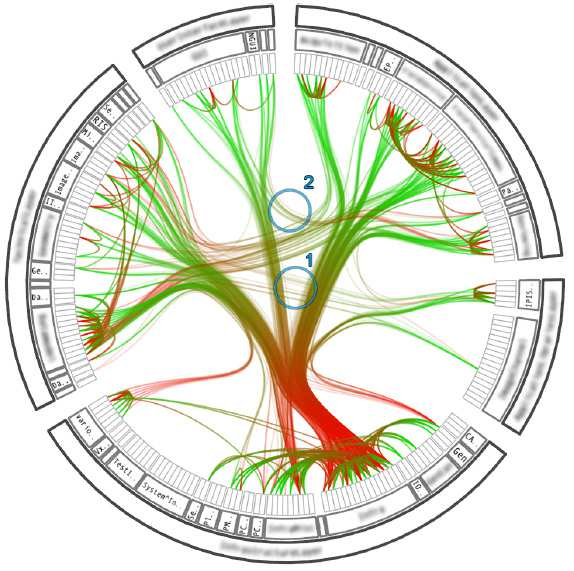
\includegraphics[width=.45\textwidth]{../figuras/hbundling.png}
  \caption[Bundling hierárquico na visualização de dados de software]{Bundling hierárquico na visualização de dados de software. As cores mapeiam
o sentido do acesso, verde é a origem, vermelho é o alvo. Fonte: \citep{Holten2006}.}
  \label{fig:bundling-hierarquico}
\end{figure}

\subsection{Modelos de \emph{Bundling}}
\label{sec:modelos-de-bundling}

  O cálculo de um \emph{bundle} não possui uma definição precisa, e por isso há
uma grande variedade de algoritmos e abordagens para modelar problemas de
agrupamento de arestas com \emph{bundling}, que podem variar significativamente
de um para outro em questões de complexidade e aplicação dos algoritmos
\citep{Zhou2013}.  \emph{Force-directed edge bundling} (FDEB), apresentado em
\citet{Holten2009}, cria \emph{bundles} através da atração entre pontos de
controle colocados ao longo das arestas e é considerado um modelo baseado em
custo, já que tenta minimizar o valor de uma função de custo que representa a
força de atração entre as arestas.  \emph{Hierarchical Edge Bundling} (HEB)
agrupa as arestas baseadas na estrutura hierárquica do grafo para o cálculo dos
\emph{bundles} e por isso é considerado um modelo geométrico \citep{Holten2006}. Outra
classificação são os modelos baseados em imagem, como \emph{Skeleton-based edge
bundling} (SBEB) e \emph{Kernel Density Estimation-based Edge Bundling}
(KDEEB), que surgiram mais recentemente. Eles utilizam algoritmos de
clusterização para extrair a estrutura geral do grafo para então calcularem os
\emph{bundles}. O algoritmo SBED utiliza o esqueleto do grafo como guias para
criar \emph{bundles} com muitas ramificações \citep{Ersoy2011}, enquanto o
KDEEB utiliza um mapa de densidade do grafo para extrair sua estrutura no
espaço da imagem \citep{Hurter2012}. A Figura \ref{fig:subfigures} dá um
exemplo da variedade de possíveis saídas geradas por diferentes algoritmos de
\emph{bundling} (FDEB, SDEB e KDEEB) aplicados nos mesmos dados.  Nesse exemplo
são usados dados de uma semana do tráfego aéreo sobre os EUA.

\begin{figure}[h!]
  \centering
  \begin{subfigure}{0.44\textwidth}
    \centering
    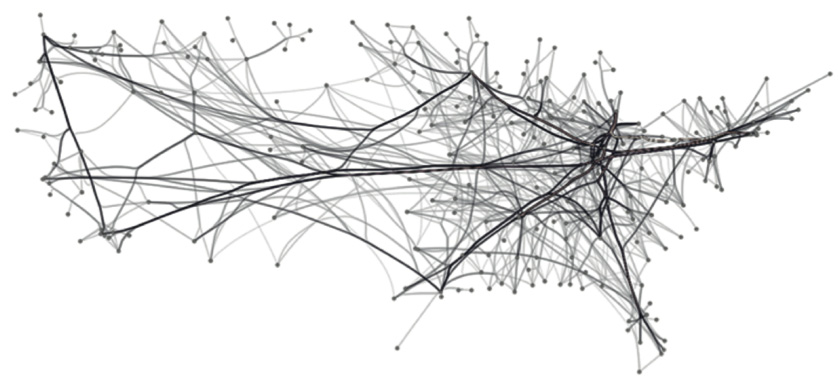
\includegraphics[width=1\textwidth]{../figuras/FDEB.png}
    \caption{FDEB}
    \label{fig:FDEB}
  \end{subfigure}

  \begin{subfigure}{0.44\textwidth}
    \centering
    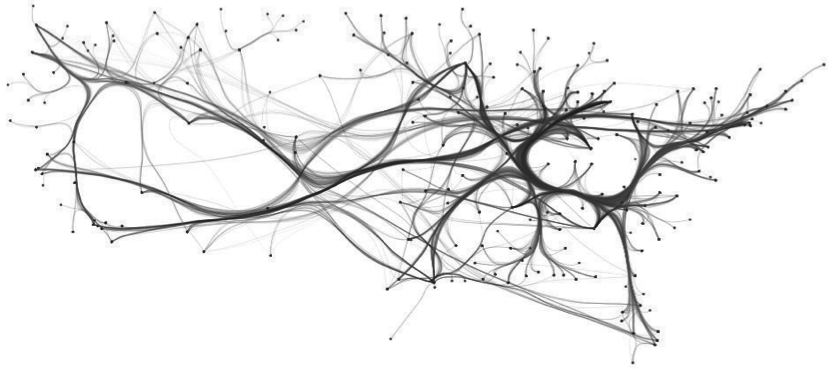
\includegraphics[width=1\textwidth]{../figuras/SBEB.png}
    \caption{SBEB}
    \label{fig:SBEB}
  \end{subfigure}

  \begin{subfigure}{0.44\textwidth}
    \centering
    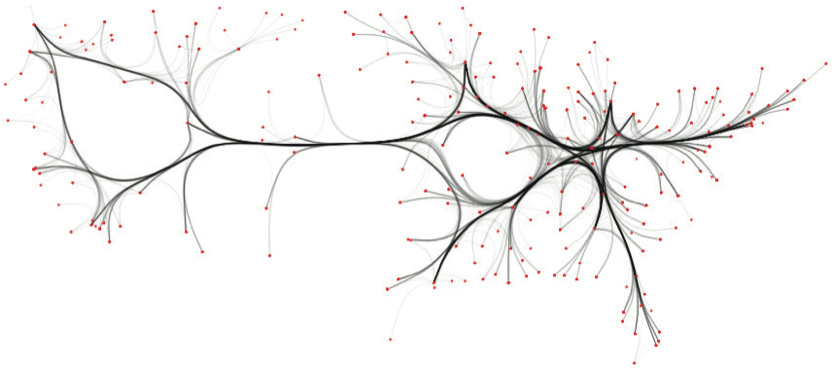
\includegraphics[width=1\textwidth]{../figuras/KDEEB.png}
    \caption{KDEEB}
    \label{fig:KDEEB}
  \end{subfigure}
  \caption[Diferentes algoritmos de \emph{bundling} aplicadas nos mesmos dados]{Diferentes algoritmos de \emph{bundling} aplicadas em dados do tráfego aéreo dos EUA - 235 nós, 2099 arestas. Fonte: \citep{Klein2014}.}
  \label{fig:subfigures}
\end{figure}

  A escolha do modelo geralmente parte da observação e experiências de
aplicação em problemas semelhantes, já que conhecer e testar diferentes
abordagens e suas variações não é uma tarefa simples. Por isso,
\citet{Lhuillier2017} recentemente propôs uma nova taxonomia para os modelos e
algoritmos de \emph{bundling} dividindo-os com base no tipo de dados em que se deseja
aplicar a técnica. Eles justificaram que desta forma pesquisadores e usuários
da técnica pudessem focar no seu contexto de aplicação e não em detalhes
específicos de implementação algorítmica. Seu estudo dividiu os modelos
existentes inicialmente em dois grupos, conforme o tipo de dados, grafos ou
trajetórias. Então, mais detalhes sobre a direção (direcionado ou não),
dimensão (2D ou 3D) e dependência do tempo (dinâmico ou estático) refinam a
divisão dentro da sua taxonomia.


\begin{figure}[!htb]
  \centering
  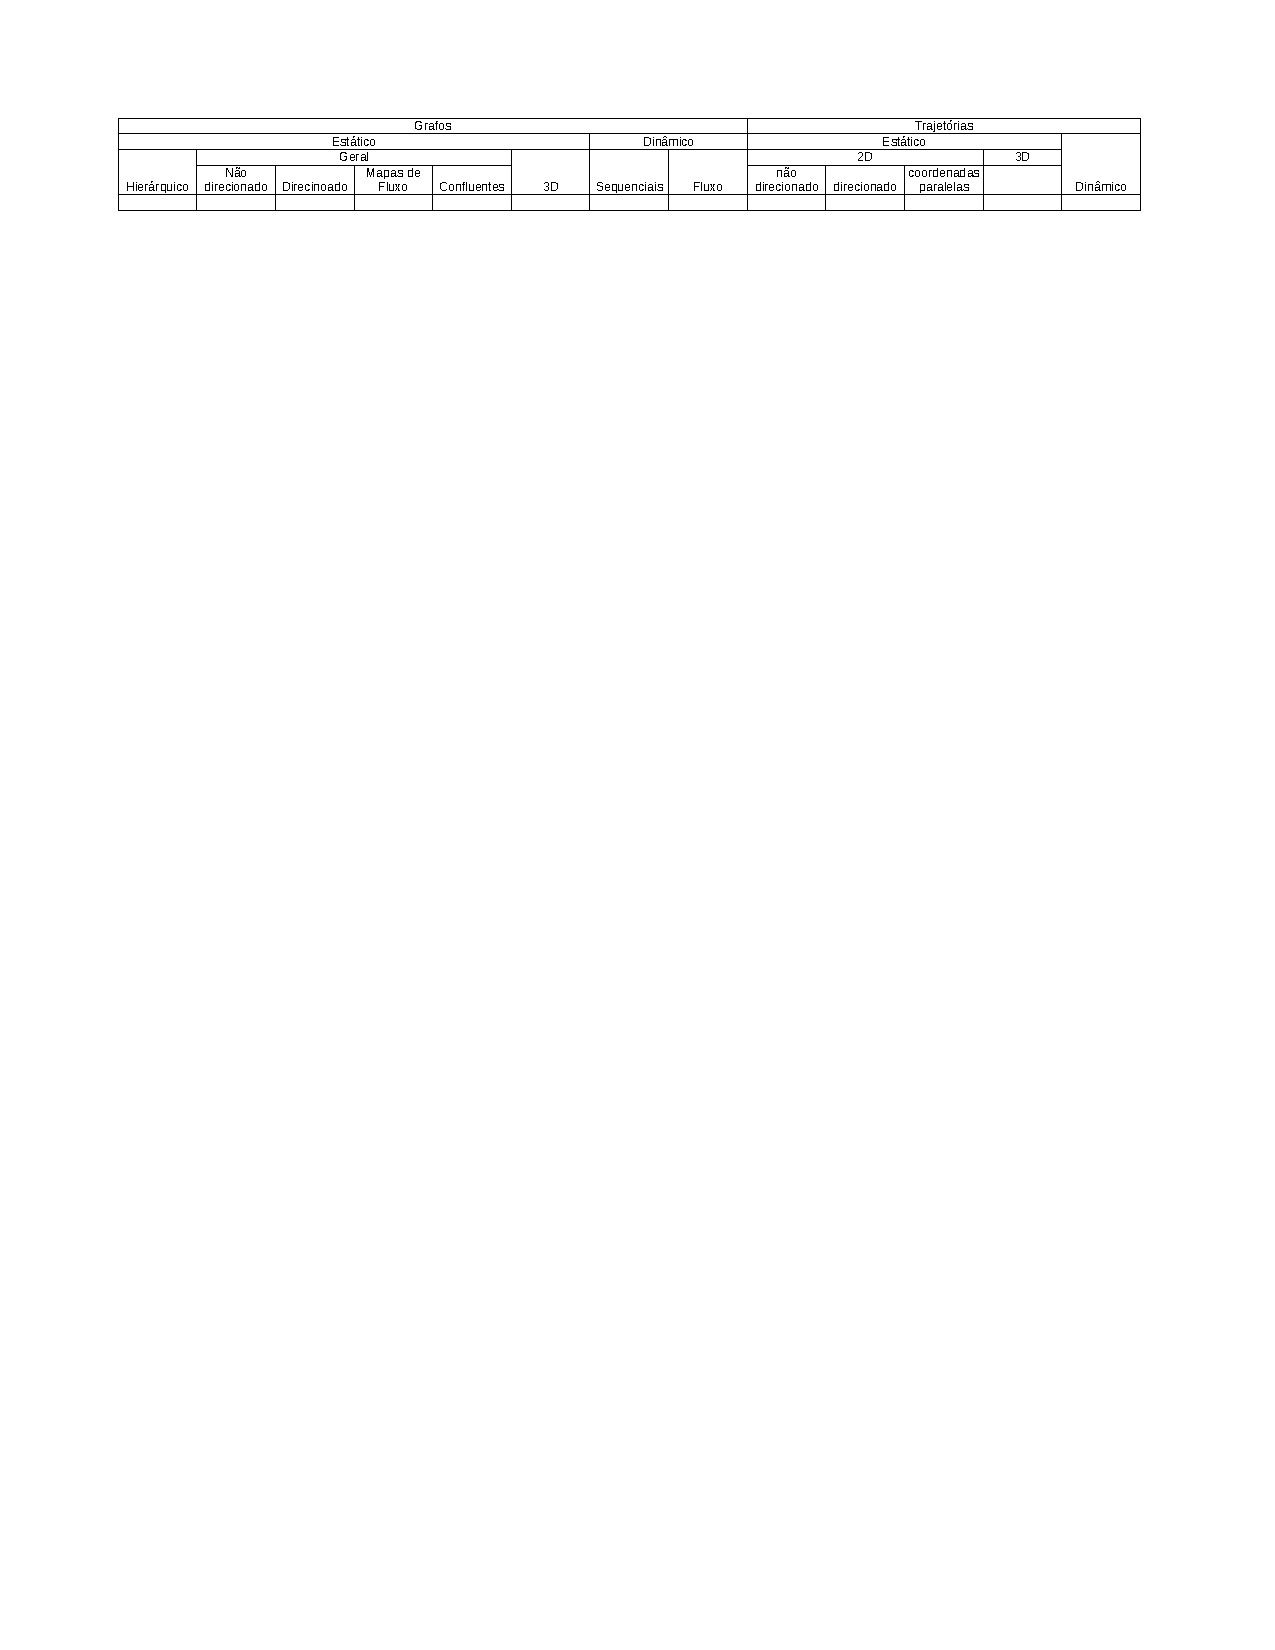
\includegraphics[width=\textwidth]{../figuras/estado-da-arte.pdf}
  \caption[Taxonomia dos métodos de \emph{bundling} baseado no tipo de dado]{Taxonomia dos métodos de \emph{bundling} baseado no tipo de dado. Fonte: \citet{Lhuillier2017}}
  \label{table:bundling-methods}
\end{figure}


Podemos então seguir a taxonomia para selecionar uma método de
\emph{bundling} que seja mais adequado para a análise de fluxos no trânsito da
cidade. \emph{Attribute-Driven Edge Bundling} (ADEB) é um algoritmo que segue um
modelo baseado em imagem e é apresentado dentro desta taxonomia como um das
opções para a análise de dados de trajetórias direcionadas. Discutimos na
próxima seção as características desse modelo e como podemos nos beneficiar
dele em nosso estudo.

\subsection{Modelo Baseado em Imagem}
\label{sec:modelo-imagem}

  Uma das etapas do \emph{bundling} é a identificação das trajetórias
similares, que requerem que cada uma delas seja comparada a todos os outras
para descobrir quais são as mais próximas, afim de agrupá-las em
\emph{bundles}.  Esse cálculo, no entanto, é bastante custoso e pode demorar
minutos em cenários com milhares de trajetórias.

\emph{Kernel Density Estimation Edge Bundling} (KDEEB) é um algoritmo proposto
por \citet{Hurter2012}. Eles observaram que ao aplicar uma operação de \emph{bundling} $B$ qualquer sobre um
grafo $G$, o resultado são áreas de maior densidade (dentro dos \emph{bundles})
e áreas de menor densidade fora deles, em comparação ao grafo original. Assim,
essa operação \emph{bundling} $B$ pode ser moldada em função de uma operação
sobre a densidade dos pontos do grafo, similar ao que faz o algoritmo de
clusterização \emph{Mean Shift} \citep{Comaniciu2012}. A partir disso, a heurística
desse algoritmo de \emph{bundling} consiste em computar repetidamente o
gradiente dos pontos em relação à uma função de densidade, e então movendo-os
para regiões mais densas apontadas pelo gradiente. O maior benefício do método
é sua implementação paralela com o uso do poder computacional de placas
gráficas (GPUs), o que levou a ganhos de desempenho de uma ordem de magnitude
em relação a métodos anteriores. KDEEB representou uma abertura para uma área
chamada \emph{image-based bundling}, ou métodos baseados em imagem, onde $B$ é
implementado via operações de processamento de imagem, diferentemente de
métodos puramente geométricos existentes até então. O algoritmo consiste nos
seguintes passos:

\begin{enumerate}
  \item Converte o grafo $G$ em um mapa de densidade usando uma função de
densidade. A função utilizada é um estimador baseado em núcleos, geralmente um
estimador Gaussiano ou Epanechnikov.

  \item Computar o gradiente da função de densidade para cada ponto/nó do
grafo. O cálculo do gradiente indica a direção onde há maior quantidade
de nós/arestas aglomeradas no grafo.

  \item Mover os nós na direção do gradiente (áreas mais densas). Essa etapa é
suavizada movendo-se os nós pela norma do gradiente, ou seja, em apenas uma unidade
a cada iteração. Isso evita que as arestas dêem grandes saltos.

  \item Corrigir distorções causadas pela movimentação dos nós com filtro
Laplaciano (opcional).  O passo anterior pode causar pequenas distorções, como
por exemplo, a sobreposição de nós. Esta é uma forma de se corrigir essas
distorções sem que se perca a estrutura geral do grafo.

  Repetir a partir do passo 1 até a convergência do algoritmo, o que leva cerca de 8..10
iterações.
\end{enumerate}

%\citet{Hurter2012} apresentam ainda uma maneira para limitar os \emph{bundles}
%com relação a obstáculos presentes no caminho das arestas. Um obstáculo
%qualquer, representado por seus limites espaciais pode ser contornado
%alterando-se a função de densidade, que sofre uma degradação dentro da área
%geométrica do obstáculo. Com isso, o gradiente age como uma força de repulsão
%das arestas que cruzam o obstáculo e faz com que as arestas sejam movidas
%na direção pra fora de suas bordas.

  {\emph{Attribute-Driven Edge Bundling} (ADEB) é uma extensão do algoritmo
KDEEB, proposta por \citet{ZegarraFlores2016}, e que permite a separação das
arestas conforme sua direção. Essa informação é obtida percorrendo cada aresta
a partir do ponto de origem até o destino e calculando para cada uma delas um
vetor unitário que aponta a sua direção, que é mapeado para o
ângulo desse mesmo vetor. Então, cria-se um mapa de densidade direcionado, onde são
consideradas apenas as arestas que vão na mesma direção (mesmo ângulo). Esse
algoritmo herda todos os benefícios de desempenho e robustez apresentados pelo
KDEEB, o que o faz um método adequado para a análise do tráfego de veículos no
trânsito da cidade.

\subsection{\emph{Bundling} em Dados Dinâmicos}

  Um grafo dinâmico é aquele no qual seus nós e arestas são dependentes do
tempo, ou seja, a cada momento \emph{t}, existe um grafo G(t) diferente a ser
explorado. Nesse contexto, dois diferentes tipos de grafos dinâmicos podem ser
considerados, grafos sequenciais e grafos de fluxo \citep{Hurter2013}. Um
grafo sequencial consiste em um conjunto de grafos $G^i = (V^i, E^i)$, onde
cada grafo $G^i$ é como um retrato no momento $i$ de um sistema que é
dependente do tempo. Grafos de fluxo, por outro lado, são definidos como um
conjunto de vértices $V$ e arestas $E$, onde as arestas são definidas pelo seu
tempo de vida e nós. Grafos de fluxo não possuem uma sequência pré-definida e
são tipicamente obtidos de fontes de dados online.

  O uso de \emph{bundling} nesse cenário é similar a outros métodos de
visualização de grafos dinâmicos. Para grafos sequenciais o \emph{bundling} é
aplicado a cada grafo $G^i$ de maneira estática. Já em grafos de fluxo, os
dados são divididos em janelas de tempo e o algoritmo é aplicado em cada
intervalo $\Delta t$, que podem ser colocados lado a lado para comparação em
uma técnica conhecida como \emph{small multiples}. Uma outra maneira de se
visualizar a dinâmica é com o uso de animações, como mostram
\citet{Hurter2014}. A vantagem desse método sobre o anterior é que ele se
adequa melhor à análise de longas séries temporais.

-----------------------------

  Os conceitos apresentados servem de base para a nossa proposta de
visualização dos dados do tráfego de veículos no trânsito. O processo de
formulação da proposta inclui a definição do tipo de visualização que iremos
utilizar, obter domínio sobre os dados do trânsito e suas propriedades, para
posteriormente chegarmos a uma análise dos fluxos de origem e destino em
diferentes níveis de detalhe a partir de um modelo de \emph{bundling}, além de
investigar formas de destacar essas propriedades dentro da visualização. No
próximo capítulo apresentamos uma revisão da literatura sobre alguns trabalhos
que utilizam \emph{bundling} e outras técnicas para análise de dados de
tráfego.
